\chapter{Results and Discussion}\label{chap:results}
% Evaluation Criteria:
% - Quality of explanation (written)
% - Support with diagrams, tables and figures
% - Table headings and figure captions
% - Clear axis labels on all figures
% - Figure complexity
% Discussion
% - Quality of explanations (written)
% - Comparison with related work
% - Discussion of implications
% - Discussion of limitations
\section{Overview}
\subsection{Recap}
\draft{Before, ....}
\todo{make quick recap on approach for who starts reading here}

\todo{add note on additives, detection if one was there in the first place: alternatively outlook}
\subsection{What's to come}
\draft{In this Chapter, ...}

\subsection{Note on differences to impl}
\todo{redo subsection titles and structure}
\textbf{Note} that while all code (refer to \secref{impl} for notes on implementation) includes \texttt{additive}, figures in this chapter do not.
This decision was made due to mistaken modeling of the task, which resulted in horrendous accuracy.
7B-sized models all had less than 1\% correct (except for Vicuna with 2.5\%), and even large models had either below 1\% or around 15\% correct (\model{llama2} and \model{falcon}, not the instruct-variant).

Instead of literal extraction, the task should have been modeled as classification task.
This was not redone due to time constraints.


\todo{build graphs for each model family -- if I have enough time for that}

\begin{figure}[!htbp]
    \begin{centering}
        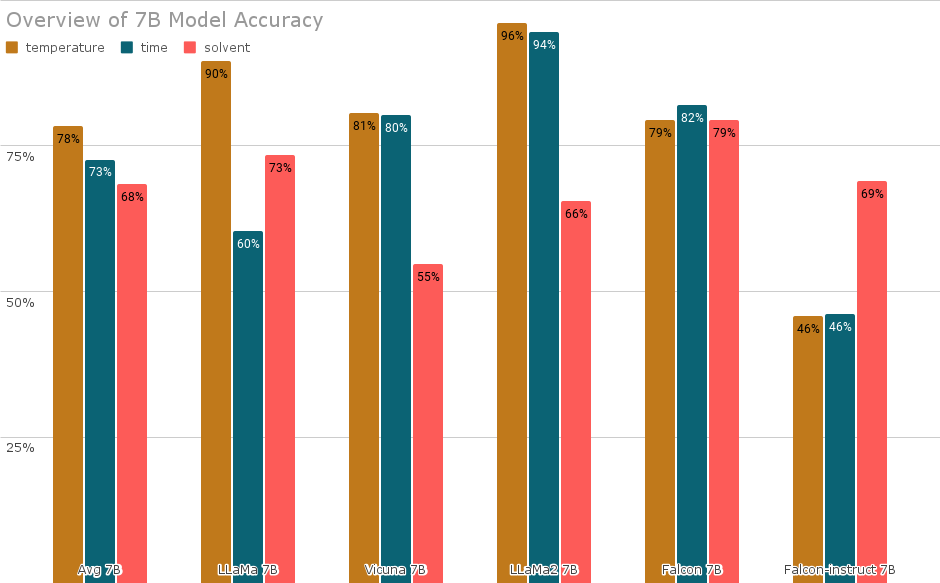
\includegraphics[width=0.9\textwidth]{img/overview_7b_accuracy}
        \caption[Overview of 7B Models Accuracy]{\textbf{Overview of the Accuracy of Models with a Size of 7B parameters.}
        On the left is the average over all 7B sized models.
        The accuracy of \ttemp and \ttime is within 3 \glspl{pp} of the other for each model except \model{llama}, where the difference is 30 \glspl{pp}.
        On average, the accuracy for \ttemp is 78\%, 73\% for \ttime, and 68\% for \tsolv.
        }
        \label{fig:7b_acc}
    \end{centering}
\end{figure}


\begin{figure}[!htbp]
    \begin{centering}
        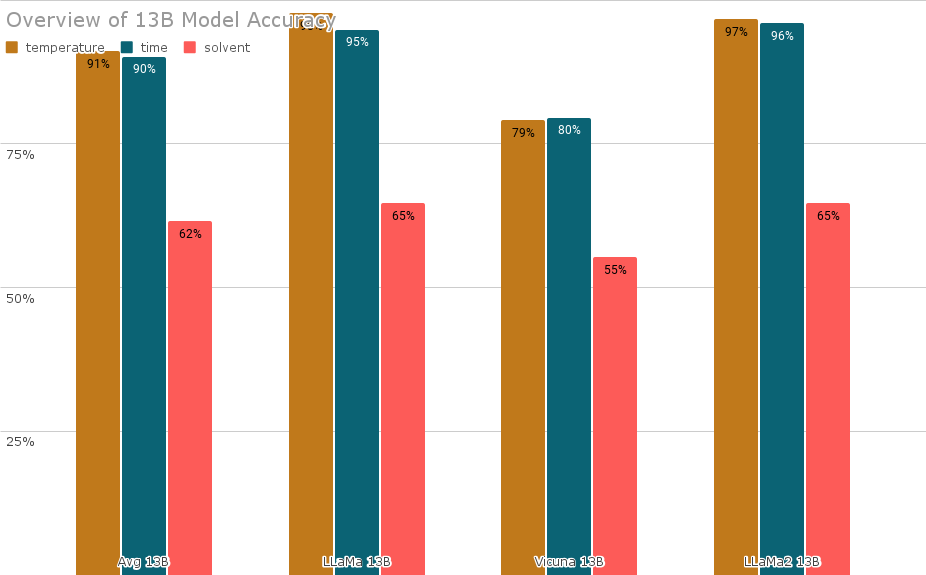
\includegraphics[width=0.9\textwidth]{img/overview_13b_accuracy}
        \caption[Overview of 13B Models Accuracy]{\textbf{Overview of the Accuracy of Models with a Size of 13B parameters.}
        Leftmost is the average over all 13B sized models.
        \model{falcon} does not have a 13B sized variant.
        On average, the accuracy for \ttemp is 90.3\%, 89.1\% for \ttime and 54.4\% for \tsolv.
        }
        \label{fig:13b_acc}
    \end{centering}
\end{figure}


\begin{figure}[!htbp]
    \begin{centering}
        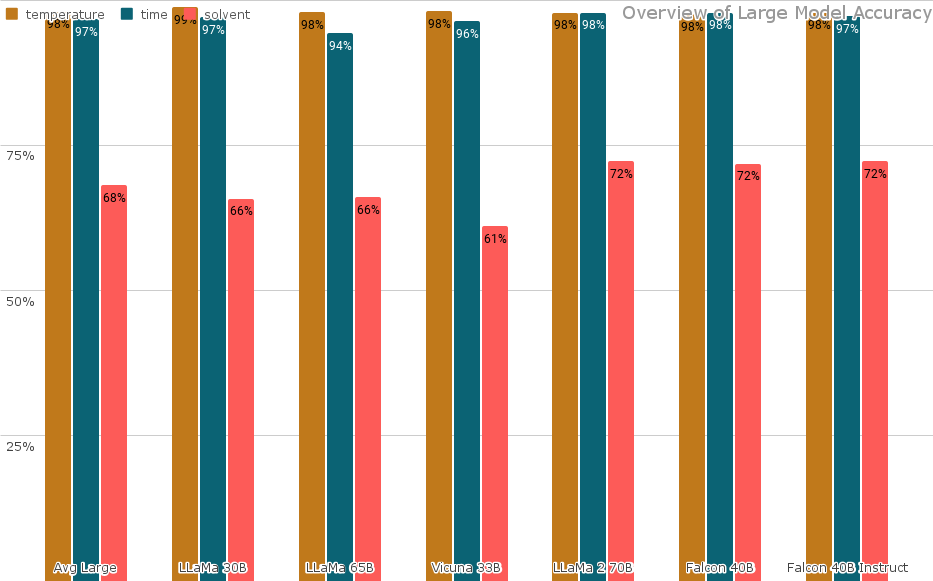
\includegraphics[width=0.9\textwidth]{img/overview_large_accuracy}
        \caption[Overview of Large Model Accuracy]{\textbf{Overview of the Accuracy of Models with a Size over 30B parameters.}
        Leftmost is the average over all models upwards of 30B parameters.
        On average, the accuracy for \ttemp is 98\%, 97\% for \ttime and 68\% for \tsolv.
        \model{llama2} does not have a 30B or 33B-sized variant.
        There is also no \model{vicuna}-65B variant made available from \gls{lmsys}.
        \model{llama2} and both \model{falcon} models achieve 72\% accuracy on \tsolv extraction, 6-11 \glspl{pp} more than other models.
        }
        \label{fig:large_acc}
    \end{centering}
\end{figure}



\section{Accuracy Overview}\label{sec:result:first}

\subsection{7B Parameter Models}\label{sub:result:7b}
As can be seen in \figref{7b_acc}, accuracy in extracting \ttemp and \ttime data varies wildly, both within and across models.

\model{llama2} has the highest accuracy for both \ttemp and \ttime, but \model{falcon} is more accurate in \tsolv prediction on our dataset.
Based on this, it seems that \model{llama2}-7B already achieves close to the highest accuracy for extraction of \ttemp, and is close behind on \ttime.

More information on why \model{llama} is so much worse in \ttime accuracy than \ttemp accuracy can be found in \subref{unitconfusion}.


\subsection{13B Parameter Models}\label{sub:result:13b}

As can be seen in \figref{13b_acc}, accuracy improved on average, but primarily for \model{llama}.
In fact, the accuracy of \model{vicuna}-13B even slightly degraded when compared to \model{vicuna}-7B on \ttemp and \ttime, and accuracy on everything mostly stayed stagnant for \model{llama2}.
\model{llama} increased accuracy on \ttemp by 6 \glspl{pp}, but particularly on \ttime by 33 \glspl{pp}.

\model{vicuna}-13B is the weakest in accuracy for \ttemp and \ttime, trailing by about 14 \glspl{pp} behind \model{llama} and \model{llama2}.
From what was seen from \model{falcon}-instruct-7B in \subref{result:7b}, \model{falcon}-instruct-13B should still be worse than \model{vicuna}-13B, but \model{falcon} does not have a 13B variant.

\subsection{Large Models}\label{sub:result:large}
As can be seen in \figref{large_acc}, scores between large models differ marginally at best.
Surprisingly, the accuracy on \tsolv extraction improved by less than maybe expected.
In fact, as can be seen in the previous \figref{7b_acc}, smaller models were in average similarly capable, though the higher variance of smaller models included those both more and less capable than its larger siblings.
This may be due to accidential sucess, and would warrant further analysis.




\section{Frequent Mistakes}\label{sec:mistakes}
Analysis of cases where the extracted data was incorrect can provide valuable insight in failure modes.
Insight on unit confusion, particularly of smaller models, is provided in \subref{unitconfusion}.
Resolution of solvents and problems with it are looked into in \subref{solv}, before \subref{oom} gives a short account of a more complex failure mode.

\subsection{Unit Confusion}\label{sub:unitconfusion}
\begin{figure}[!htb]
    \begin{centering}
        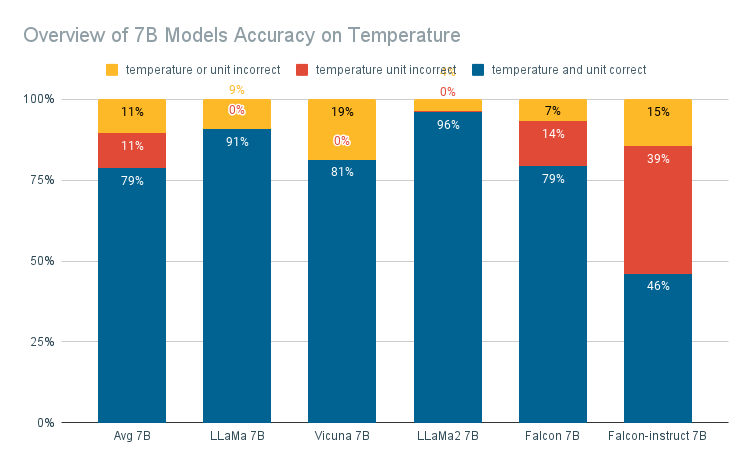
\includegraphics[width=\textwidth]{img/overview_7b_temp}
        \caption[7B Models Detailed Temperature Accuracy]{\textbf{Detailed Overview of 7B Models Accuracy on Temperature.}}
        On average, 7B sized models had an accuracy of 78\% on the extraction of the \ttemp the synthesis was run at.
        Most models did not have problems with temperature units, apart from \model{falcon}.
        \label{fig:7b_temp}
    \end{centering}
\end{figure}

\begin{figure}[!htb]
    \begin{centering}
        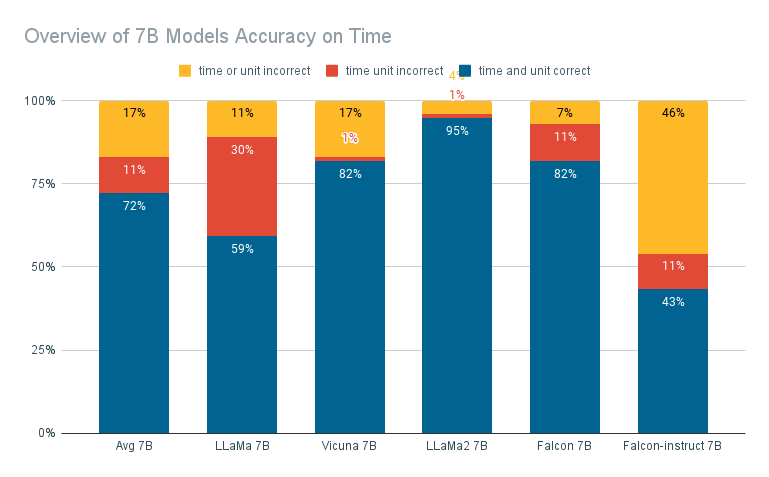
\includegraphics[width=\textwidth]{img/overview_7b_time}
        \caption[7B Models Detailed Time Accuracy]{\textbf{Detailed Overview of 7B Models Accuracy on Time.}
            On average, 7B sized models had an accuracy of 72\% on the extraction of the synthesis duration, and a third of the mistakes (11\% of 28\% total mistakes), were simply due to getting the unit of the duration wrong.
            \model{llama} struggled the most, providing inaccurate units for about a third of all answers on \ttime.
            Both \model{falcon} and \model{falcon}-instruct confused units in about 11\% of answers.
            However, \model{vicuna} and \model{llama2} gave the wrong unit in only 1\% of cases.
        }
        \label{fig:7b_time}
    \end{centering}
\end{figure}

\begin{figure}[!htbp]
    \begin{centering}
        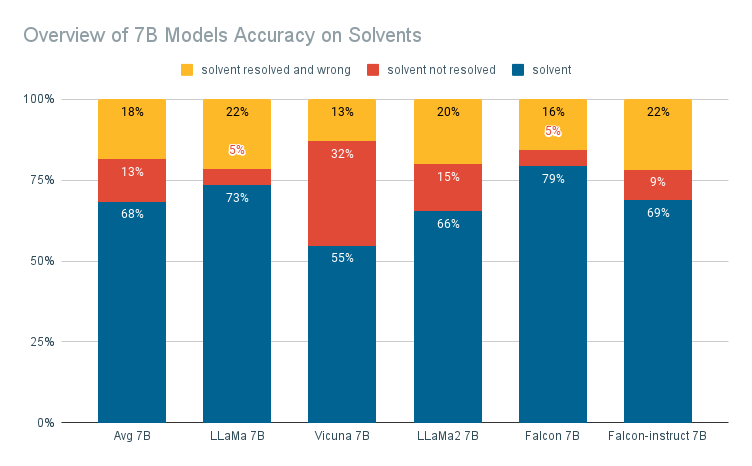
\includegraphics[width=\textwidth]{img/overview_7b_solv}
        \caption[7B Models Detailed Solvent Accuracy]{\textbf{Detailed Overview of 7B Models Accuracy on Solvents.}
            On average, accuracy on \tsolv was 68\%, and an additional 13\% could not be resolved.
            \model{llama}-7B and \model{falcon}-7B had the fewest unresolved answers, at 5\% each.
        }
        \label{fig:7b_solv}
    \end{centering}
\end{figure}

\begin{figure}[!htb]
    \begin{centering}
        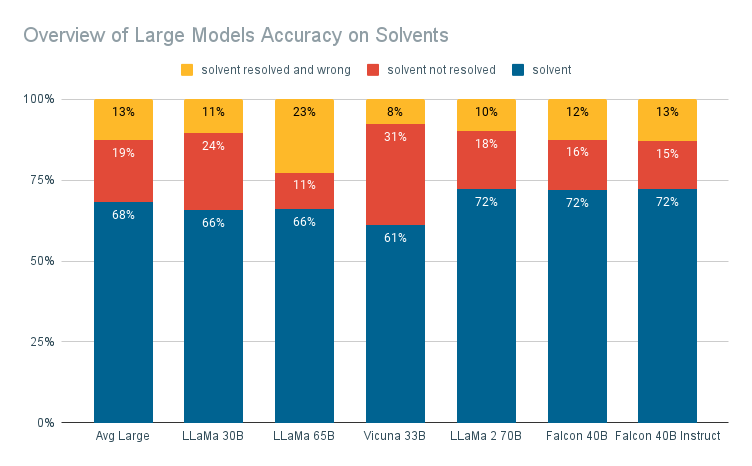
\includegraphics[width=\textwidth]{img/overview_large_solv}
        \caption[Large Models Detailed Solvent Accuracy]{\textbf{Detailed Overview of Accuracy from Models with a Size over 30B parameters on Solvents.}
            On average, accurcy on \tsolv was 68\%, and an additional 19\% could not be resolved. The remaining 13\% resolved to a compound not used as \tsolv.
        }
        \label{fig:large_solv}
    \end{centering}
\end{figure}

One interesting observation is that smaller models appear to make a lot of `easy' mistakes.
Not all such simple mistakes can be easily classified, but mistakenly outputting the wrong unit can.
For \textit{unit confusion}, the following instances where counted: the answer (on \ttemp or \ttime) provided from a model is wrong, but interpreting the same answer with a different unit could get the correct answer.
More details on model output structure can be found in \secref{prompts}.

For example, in one instances \model{falcon} confidently answered 20 °K, when the correct answer would have been 20 °C.

\paragraph{Temperature Units}
As can be seen in \figref{7b_temp}, only \model{falcon} experiences unit confusion for temperature -- and in particular the instruct-variant.
It is unclear why that might be the case exactly, but it seems to be in part of the dataset \model{falcon} was trained on.

\paragraph{Time Units}
Unit confusion on \ttime seems to affect all models to some degree, as can be seen in \figref{7b_time}.
Interestingly, \model{llama} seems to be affected the most, followed by \model{falcon}.
This also explains how \model{llama} could quickly gain 33 \glspl{pp} in accuracy between sizes 7B and 13B (Compare \figref{7b_acc} and \figref{13b_acc}) -- mostly due to using correct time units.

\paragraph{Bigger-sized Models}
Unit confusion on models sized 13B parameters or more is happening in less than 0.5\% of cases (in 0-4 answers of 778 data points), and is thus of no further interest.


\subsection{Solvent Resolution}\label{sub:solv}
As mentioned previously in \subref{compsolv}, compounds may have multiple names that are used in different synthesis paragraphs, but not all of them may get resolved from \texttt{pubchempy}.
Thus, taking a closer look at how often answers for \tsolv from 7B-sized models could not be resolved in \figref{7b_solv} reveals an interesting picture.

First, all models seem to be affected by not being able to resolve \tsolv to some degree.
The previously mentioned case of `distilled H2O' not resolving albeit clearly occuring in eight synthesis paragraphs as solvent, indicates that at least some of the answers provided by models may be, in fact, correct.
However, this is probably not the case for most of the answers provided by \model{vicuna}-7B, where about 31\% of answers did not resolve.
This also indicates that the approach taken for compound resolution in this work can be improved.

Second, larger models seem to be affected even more, as can be seen in \figref{large_solv}.
One hypothesis for this observation is that the models are more accurate, and quote the correct \tsolv verbatim, but the answer cannot be resolved.
This may be true in particular for the \tsolv \texttt{N,N-DIMETHYLACETAMIDE}, where the synthesis paragraphs contain none of its 125 synonyms in 34 cases (or about 3.76\% of the dataset).

\subsection{Orders of Magnitude}\label{sub:oom}
In some cases, the following mistake was observed:
answers of \ttime where clearly supposed to be in seconds (e.g. 864000 seconds are ten days), but the number of zeroes was off by one.
A similar mistake happened sometimes with \ttemp units in Kelvin.
This did not preclude the unit from being wrong.
In fact, it sometimes appears that (since the unit information is generated later) the model attempted to increase or decrease its previous answer with a different unit than would be expected, making it closer to correct than simply having the wrong number of zeros -- but still wrong.
% As if trying to make up for that, the provided unit (probably because it was generated later) was sometimes \textit{inbetween} of what it 
Smaller models seem to have a higher tendency of making these mistakes, but no further analysis was done due to time constraints.



% \section{Additional Observations}\label{sec:discussion}
% There are two interesting trends that can be observed across models:
% 
% \begin{enumerate}
%     \item Larger models are more accurate in the extraction of \ttemp and \ttime.
%     \item Accuracy in the extraction of \tsolv appears to be largely independent of model size.
% \end{enumerate}
% 
% The first observation confirms general expectations.
% However, even 13B-sized \model{llama} and \model{llama2} are only marginally worse than any of their bigger siblings, which indicates that even mid-sized models might already be fully capable of the extraction of parameters such as \ttemp and \ttime.
% 
% The second observation, that models mostly achieve the same accuracy on \tsolv extraction regardless of size, is indicative of 
% the models getting \textit{confused} rather than fundamentally being incapable of doing it.
% The accuracy of just shy of 60\% also indicates that \textit{for the most part} it is clear what the task is.
% This suggests that this task could benefit substantially from additional prompt engineering, and maybe even more from fine-tuning. See \secref{out:prompt} and \secref{out:sft} for the outlook on each respectively.


% Some of the answers given are hilarious too \todo{put some example hallucinations in the results chapter}

% \verb!2023-09-09 16:05:36 ERROR    pcp: Could not find `cid` for [distilled H2O]!


\section{Supervised Fine Tuning}\label{sec:sft}
Pretrained \glspl{LLM} are trained on so much data that they become generally capable of most tasks even with no additional fine-tuning \cite{brown_language_2020}, but this usually takes many thousands of GPU-hours \cite{touvron_llama_2023, scao_what_2022}.
Instead, fine-tuning a pretrained model has substantial benefits: it requires many orders of magnitude fewer GPU-hours, and sometimes more importantly, a lot fewer examples for training to achieve similar results to a specifically trained model for most tasks \cite{gaddipati_comparative_2020}.

More information on pre-training a \gls{LLM} can be found in \secref{training}, and \subref{finetune} has additional details on fine-tunig.

In the end, fine-tuning was abandoned for this work due to lack of success and time constraints. See \secref{con:sft} for conclusions and \secref{out:sft} for an outlook on comparisons with fine-tuned models.

What follows are two excerpts of what was encountered when attempting to fine-tune \glspl{LLM} using th \gls{transformers} library.
These excerpts are by no means exhaustive, as many hours of bugfixing where necessary to even get to these points.
Further hours, while sometimes yielding different errors, yielded no additional results or insight.
Neither did interacting with the community, where a number of people had slightly different but very similar problems, almost always with no answer in any official or unofficial forum.

% Other failed attempts tended to follow similar patterns of:
% 
% \begin{itemize}
%     \item Example demonstrated in official documentation, but individual parts have no documentation available.
%     \item Straightforward attempts to slightly adjust official examples fails due to hidden complexity the short and elegant example abstracted away.
%     \item The error is very obscure and far removed from the actual configuration.
%     \item \textit{Some} information can be found in official and unofficial forums, blog posts, and source code. Most of the time, it's other people with the same problem and no solution.
% \end{itemize}


\subsection{Excerpt 1: Broken Models}\label{sub:brokenft}
Since for this work a custom dataset is used, it also requires a custom dataloader.
Traditionally, specifically for training, a dataloader contains one field for the 'input' of the model, and one for the label, or 'output' of the model, the optimizer should optimize for as a result of the input.
Each item of the dataloader is a dictionary of keys, with specific keys for input and output.
There is however, only partial and very conflicting documentation on the existance and usage of these keys.

% \todo{continue writing excerpt 1 from here on}
Additionally, \glspl{LLM} require input to be converted to tokens before being able to process it.
In the various examples that can be found, three main keys are of primary importance for dataloaders for \glspl{LLM}:

\begin{itemize}
    \item \mpy{"input_ids"}
    \item \mpy{"attention_mask"}
    \item \mpy{"labels"}
\end{itemize}

\code{input.py}{input}{Excerpt of what could be found in a custom dataloader. \mpy{text} describes any string the model may be provided as input. The tokenizer converts any string to a list of tokens and an attention mask, among other things.
}

However, none of these is properly documented or explained.
The common usage of the keys \mpy{"input_ids"} and \mpy{"attention_mask"} is rather straightforward, and few working examples show anything different to what can be seen in \coderef{input}.
Despite that, \mpy{"label"} is not so clear.

Since neither of the three is documented, what remains is looking at use from others, or digging into the code.
Multiple tutorials and even official sources (e.g. microsoft \cite{deepspeedexamples_2023}), use it in the following way: \mpy{"label": text_encodings["input_ids"]}.

This, in fact, can train a model and result in model weights differing from the original ones.
However, this now trained model was broken, as it did not generate anything that was not an \mpy{"<EOS>"}-token.
These tokens are usually used as a stopping criterion during generation -- meaning that the model predicts that a natural seperation happens between the previous and the next tokens. 
This is true in cases where \mpy{"<EOS>"} denotes a switch from user-generated to assistent-generated text, a paragraph or answer ended or similar (as it will be used in training data).
Nonetheless, this is not the case here. Even when ignoring the \textit{first} such token, no further \mpy{"<EOS>"}-tokens should follow immediately after.

At this point, it is unclear what exactly happened.
Looking through source code of used modules from the \gls{transformers} library provided little insight.
The main hypothesis for the failure is that the optimizer trained the model that \textit{no additional output} is required, since both \mpy{"input_ids"} and \mpy{"label"} where equal.
However, this approach seems to work for other groups in certain circumstances, which substantially reduces the credibility of the hypothesis.
So far, no other potential explanation has been found.

Additionally, attempts at mask manipulation were not possible due to the nature of \gls{causal} which all \glspl{LLM} are.
Other sources tokenize different text for \mpy{"label"}, though this is more rare and exact usage is inconsistent.
No further attempts at this approach where made due to focusing on other, seemingly more promising venues.


\subsection{Excerpt 2: Broken Libraries}\label{sub:libraries}
Another attempt made use of the high-level \gls{hf} \texttt{trl} (Transformer Reinforcement Learning) library, purpose-built for use-cases of (supervised) fine-tuning.

\begin{sloppypar}
The couple of examples provided, while working with only a few lines of code, obscure the complex and undocumented inner workings of the library.
Usually, a \texttt{DataCollator} is used to batch-process multiple items from the dataloader, and items from the dataloader are already tokenized.
However, the in examples used but otherwise undocumented \texttt{DataCollatorForCompletionOnlyLM} (or more specifically, the underlying \texttt{DataCollatorForLanguageModeling}) attempts to abstract away the process of tokenization, so that any dataloader providing text samples could be used, independent of tokenization.
This abstraction would generally reduce redundant boilerplate code.
\end{sloppypar}

\code{error.py}{error}{Counterintuitively, this is not a \mpy{KeyError}.}

\begin{sloppypar}
After inspecting some of the working examples to learn that the dataloaders provided a \mpy{"text"}-key, and adapting other code accordingly to \textit{not} tokenize it beforehand, this resultet in a \mpy{ValueError} missing \mpy{"input_ids"}, as can be seen in the full message in \coderef{error}.
When instead tokenizing before the \texttt{DataCollatorForCompletionOnlyLM}, it would fail, complaining that it will do tokenization itself.
\end{sloppypar}

% \subsection{Community Support}
